\documentclass[11pt,letterpaper]{article}

% =============================================================================
% PACKAGES
% =============================================================================
\usepackage[margin=1in]{geometry}
\usepackage{enumitem}
\usepackage{setspace}
\usepackage{graphicx}
\usepackage{xcolor}
\usepackage{amssymb}
\usepackage{tikz}
\usetikzlibrary{shapes.geometric, shapes.misc, arrows.meta, positioning, fit, backgrounds, calc, decorations.pathreplacing, shapes.symbols}
\usepackage{tcolorbox}
\usepackage{booktabs}
\usepackage{longtable}
\usepackage{array}
\usepackage{tabularx}
\usepackage{multirow}
\usepackage{fancyhdr}
\usepackage{titlesec}
\usepackage[colorlinks=true,linkcolor=blue!60!black,urlcolor=blue!60!black,citecolor=blue!60!black]{hyperref}
\usepackage{bookmark}
\usepackage{parskip}
\usepackage{float}
\usepackage{caption}
\usepackage{subcaption}
\usepackage{listings}
\usepackage{microtype}

% =============================================================================
% CONFIGURATION
% =============================================================================
\setstretch{1.15}

% Define colors
\definecolor{primary}{RGB}{0, 73, 135}
\definecolor{secondary}{RGB}{70, 130, 180}
\definecolor{accent}{RGB}{220, 100, 50}
\definecolor{lightgray}{RGB}{245, 245, 245}
\definecolor{darkgray}{RGB}{80, 80, 80}
\definecolor{nodecolor}{RGB}{230, 242, 255}
\definecolor{componentcolor}{RGB}{255, 248, 220}
\definecolor{connectorcolor}{RGB}{220, 255, 220}

% Section formatting
\titleformat{\section}{\Large\bfseries\color{primary}}{\thesection}{1em}{}[\titlerule]
\titleformat{\subsection}{\large\bfseries\color{secondary}}{\thesubsection}{1em}{}
\titleformat{\subsubsection}{\normalsize\bfseries\color{darkgray}}{\thesubsubsection}{1em}{}

% Header/Footer
\pagestyle{fancy}
\fancyhf{}
\fancyhead[L]{\small\textcolor{darkgray}{Deployment Viewpoint Specification}}
\fancyhead[R]{\small\textcolor{darkgray}{Architecture Documentation}}
\fancyfoot[C]{\thepage}
\renewcommand{\headrulewidth}{0.4pt}

% Custom environments
\newtcolorbox{definitionbox}[1][]{
    colback=lightgray,
    colframe=primary,
    fonttitle=\bfseries,
    title=#1,
    boxrule=0.5pt,
    arc=2pt,
    left=8pt,
    right=8pt,
    top=6pt,
    bottom=6pt
}

\newtcolorbox{examplebox}[1][]{
    colback=white,
    colframe=secondary,
    fonttitle=\bfseries,
    title=#1,
    boxrule=0.5pt,
    arc=2pt,
    left=8pt,
    right=8pt,
    top=6pt,
    bottom=6pt
}

\newtcolorbox{warningbox}[1][]{
    colback=orange!5,
    colframe=accent,
    fonttitle=\bfseries,
    title=#1,
    boxrule=0.5pt,
    arc=2pt,
    left=8pt,
    right=8pt,
    top=6pt,
    bottom=6pt
}

\newtcolorbox{guidancebox}[1][]{
    colback=green!5,
    colframe=green!50!black,
    fonttitle=\bfseries,
    title=#1,
    boxrule=0.5pt,
    arc=2pt,
    left=8pt,
    right=8pt,
    top=6pt,
    bottom=6pt
}

% Listings configuration
\lstset{
    basicstyle=\ttfamily\small,
    backgroundcolor=\color{lightgray},
    frame=single,
    framerule=0.5pt,
    rulecolor=\color{darkgray},
    breaklines=true,
    captionpos=b,
    tabsize=2
}

% Table column types
\newcolumntype{L}[1]{>{\raggedright\arraybackslash}p{#1}}
\newcolumntype{C}[1]{>{\centering\arraybackslash}p{#1}}
\newcolumntype{R}[1]{>{\raggedleft\arraybackslash}p{#1}}

% =============================================================================
% DOCUMENT BEGIN
% =============================================================================
\begin{document}

% -----------------------------------------------------------------------------
% TITLE PAGE
% -----------------------------------------------------------------------------
\hypersetup{pageanchor=false}
\begin{titlepage}
    \centering
    \vspace*{2cm}
    
    {\Huge\bfseries\color{primary} Deployment Viewpoint\par}
    \vspace{0.5cm}
    {\Large\color{secondary} Architecture Viewpoint Specification\par}
    
    \vspace{1.5cm}
    
    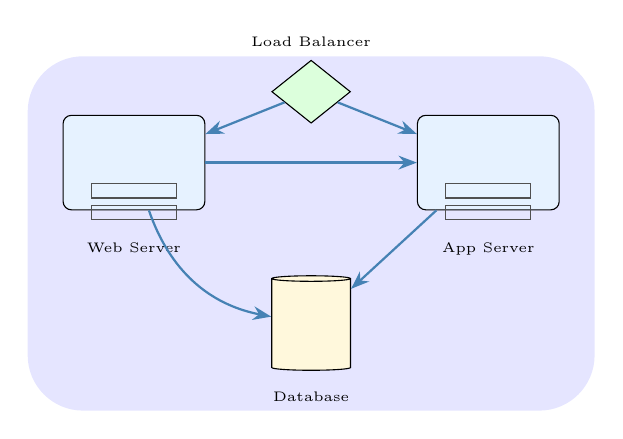
\begin{tikzpicture}[scale=0.9]
        % Background cloud shape
        \fill[blue!10, rounded corners=20pt] (-4,-2) rectangle (4,3);
        
        % Server nodes
        \node[draw, fill=nodecolor, rounded corners=3pt, minimum width=1.8cm, minimum height=1.2cm] (server1) at (-2.5, 1.5) {};
        \draw[darkgray] (-3.1, 1.2) rectangle (-1.9, 1.0);
        \draw[darkgray] (-3.1, 0.9) rectangle (-1.9, 0.7);
        \node[below, font=\tiny] at (-2.5, 0.5) {Web Server};
        
        \node[draw, fill=nodecolor, rounded corners=3pt, minimum width=1.8cm, minimum height=1.2cm] (server2) at (2.5, 1.5) {};
        \draw[darkgray] (1.9, 1.2) rectangle (3.1, 1.0);
        \draw[darkgray] (1.9, 0.9) rectangle (3.1, 0.7);
        \node[below, font=\tiny] at (2.5, 0.5) {App Server};
        
        % Database
        \node[draw, fill=componentcolor, cylinder, shape border rotate=90, aspect=0.3, minimum height=1.2cm, minimum width=1cm] (db) at (0, -0.8) {};
        \node[below, font=\tiny] at (0, -1.6) {Database};
        
        % Connections
        \draw[-{Stealth}, thick, secondary] (server1) -- (server2);
        \draw[-{Stealth}, thick, secondary] (server2) -- (db);
        \draw[-{Stealth}, thick, secondary] (server1) to[bend right=30] (db);
        
        % Load balancer
        \node[draw, fill=connectorcolor, diamond, minimum width=1cm, minimum height=0.8cm] (lb) at (0, 2.5) {};
        \node[above, font=\tiny] at (0, 3.0) {Load Balancer};
        
        \draw[-{Stealth}, thick, secondary] (lb) -- (server1);
        \draw[-{Stealth}, thick, secondary] (lb) -- (server2);
    \end{tikzpicture}
    
    \vspace{2cm}
    
    \begin{tabular}{ll}
        \textbf{Version:} & 2.0 \\
        \textbf{Status:} & Release \\
        \textbf{Classification:} & ISO/IEC/IEEE 42010 Compliant \\
        \textbf{Last Updated:} & \today \\
    \end{tabular}
    
    \vfill
    
    {\small Based on the Views and Beyond approach to software architecture documentation}
    
\end{titlepage}
\hypersetup{pageanchor=true}
\clearpage

% -----------------------------------------------------------------------------
% TABLE OF CONTENTS
% -----------------------------------------------------------------------------
\tableofcontents
\newpage

% =============================================================================
% SECTION: VIEWPOINT NAME
% =============================================================================
\section{Viewpoint Name}

\begin{definitionbox}[Viewpoint Identification]
\begin{tabular}{@{}L{3.5cm}L{10cm}@{}}
\textbf{Name:} & Deployment Viewpoint \\[0.5em]
\textbf{Synonyms:} & Installation Viewpoint, Physical Viewpoint, Infrastructure Viewpoint, Allocation Viewpoint, Deployment View, Physical Architecture View, Infrastructure View, Runtime Environment View \\[0.5em]
\textbf{Identifier:} & VP-DEPLOY-001 \\[0.5em]
\textbf{Version:} & 2.0 \\
\end{tabular}
\end{definitionbox}

\subsection{Viewpoint Classification}

The Deployment Viewpoint belongs to the \textbf{Allocation Style} family within the Views and Beyond approach. It specifically addresses the mapping between software elements and the environmental structures (hardware, networks, file systems, and runtime platforms) in which the software executes. This viewpoint bridges the gap between logical software architecture and physical infrastructure architecture.

\begin{table}[H]
\centering
\caption{Viewpoint Classification Taxonomy}
\begin{tabular}{@{}L{4cm}L{10cm}@{}}
\toprule
\textbf{Attribute} & \textbf{Value} \\
\midrule
Style Family & Allocation Styles \\
Primary Focus & Runtime Infrastructure Mapping \\
Abstraction Level & Physical/Environmental \\
Temporal Perspective & Execution Time \\
Related Styles & Work Assignment, Implementation, Install \\
IEEE 42010 Category & Environmental Viewpoint \\
\bottomrule
\end{tabular}
\end{table}

% =============================================================================
% SECTION: OVERVIEW
% =============================================================================
\section{Overview}

The Deployment Viewpoint provides a comprehensive framework for documenting how software elements are allocated to hardware resources and execution environments. This viewpoint is essential for understanding, analyzing, and communicating the physical manifestation of a software system within its operational context.

\subsection{Purpose and Scope}

The primary purpose of this viewpoint is to establish a clear mapping between software artifacts (components, modules, processes, threads) and the hardware/infrastructure elements (servers, containers, virtual machines, network devices) on which they execute. This mapping is fundamental to understanding system behavior, performance characteristics, security boundaries, and operational concerns.

\begin{definitionbox}[Viewpoint Definition]
The Deployment Viewpoint defines the correspondence between software elements of the system architecture and elements of a platform or environment model in which the software executes. It shows how software is distributed across computing nodes and how these nodes are interconnected through network infrastructure.
\end{definitionbox}

\subsection{Key Characteristics}

The Deployment Viewpoint exhibits several distinctive characteristics that differentiate it from other architectural viewpoints:

\textbf{Multi-dimensional Mapping:} Unlike simpler viewpoints that focus on a single type of relationship, the Deployment Viewpoint captures multiple simultaneous mappings---software to hardware, processes to runtime environments, data to storage systems, and communication to network infrastructure.

\textbf{Runtime Focus:} This viewpoint is concerned exclusively with the system as it exists during execution, rather than during development or build time. It captures the dynamic allocation of software to resources and the relationships that exist when the system is operational.

\textbf{Environmental Integration:} The viewpoint explicitly incorporates environmental elements that are typically external to the software architecture itself, including operating systems, middleware platforms, container orchestration systems, and cloud infrastructure services.

\textbf{Quality Attribute Implications:} Deployment decisions have profound implications for numerous quality attributes including performance, availability, security, scalability, and maintainability. This viewpoint makes these implications explicit and analyzable.

\subsection{Relationship to Other Viewpoints}

The Deployment Viewpoint does not exist in isolation but has important relationships with other architectural viewpoints:

\begin{table}[H]
\centering
\caption{Relationships to Other Viewpoints}
\begin{tabular}{@{}L{3.5cm}L{10.5cm}@{}}
\toprule
\textbf{Viewpoint} & \textbf{Relationship} \\
\midrule
Component-and-Connector & Software components identified in C\&C views are the elements being deployed. Runtime connections inform network topology requirements. \\
\addlinespace
Module & Module structure influences packaging and deployment unit boundaries. Build outputs become deployment artifacts. \\
\addlinespace
Concurrency & Process and thread structures are allocated to execution environments. Concurrency strategies affect node allocation. \\
\addlinespace
Information/Data & Data stores are mapped to storage infrastructure. Data flow paths influence network design. \\
\addlinespace
Security & Security domains map to network segments. Trust boundaries align with deployment boundaries. \\
\addlinespace
Operational & Deployment topology enables or constrains operational procedures. Recovery strategies depend on deployment architecture. \\
\bottomrule
\end{tabular}
\end{table}

% =============================================================================
% SECTION: CONCERNS
% =============================================================================
\section{Concerns}

This section enumerates the architectural concerns that the Deployment Viewpoint is designed to address. These concerns represent the fundamental questions that stakeholders have about the system's physical architecture and infrastructure.

\subsection{Primary Concerns}

\begin{enumerate}[label=\textbf{C\arabic*:}, leftmargin=2.5em]
    \item \textbf{Hardware Resource Allocation}
    \begin{itemize}[nosep]
        \item What hardware resources (servers, storage, network devices) does the system require?
        \item How are software components allocated to specific hardware resources?
        \item What are the resource requirements (CPU, memory, storage, bandwidth) for each allocation?
        \item How do hardware capabilities constrain software functionality?
    \end{itemize}
    
    \item \textbf{Network Topology and Communication}
    \begin{itemize}[nosep]
        \item How are hardware nodes interconnected?
        \item What network protocols are used for communication between nodes?
        \item What are the bandwidth and latency characteristics of network connections?
        \item How does network topology support or constrain software communication patterns?
    \end{itemize}
    
    \item \textbf{Performance and Scalability}
    \begin{itemize}[nosep]
        \item How does deployment topology affect system performance?
        \item What are the bottlenecks in the current deployment configuration?
        \item How can the system scale horizontally and vertically?
        \item What load balancing and traffic distribution strategies are employed?
    \end{itemize}
    
    \item \textbf{Availability and Reliability}
    \begin{itemize}[nosep]
        \item How does the deployment architecture support high availability?
        \item What redundancy mechanisms are in place?
        \item How are failover and recovery procedures implemented?
        \item What are the single points of failure in the deployment?
    \end{itemize}
    
    \item \textbf{Security and Isolation}
    \begin{itemize}[nosep]
        \item How are security zones and trust boundaries implemented?
        \item What network segmentation strategies are employed?
        \item How is access to infrastructure resources controlled?
        \item What encryption is applied to data in transit and at rest?
    \end{itemize}
    
    \item \textbf{Operational Management}
    \begin{itemize}[nosep]
        \item How is the system deployed and updated?
        \item What monitoring and observability infrastructure is in place?
        \item How are logs collected and aggregated?
        \item What configuration management approaches are used?
    \end{itemize}
    
    \item \textbf{Cost and Resource Efficiency}
    \begin{itemize}[nosep]
        \item What are the infrastructure costs associated with the deployment?
        \item How efficiently are resources utilized?
        \item What opportunities exist for cost optimization?
        \item How do different deployment options compare in terms of total cost of ownership?
    \end{itemize}
    
    \item \textbf{Compliance and Regulatory Requirements}
    \begin{itemize}[nosep]
        \item What geographic constraints apply to data and processing?
        \item How does deployment satisfy regulatory requirements?
        \item What audit trails and compliance controls are implemented?
        \item How are data sovereignty requirements addressed?
    \end{itemize}
\end{enumerate}

\subsection{Concern-Quality Attribute Mapping}

The following table maps deployment concerns to the quality attributes they most directly influence:

\begin{table}[H]
\centering
\caption{Concern to Quality Attribute Mapping}
\small
\begin{tabular}{@{}L{3.8cm}C{1.2cm}C{1.2cm}C{1.2cm}C{1.2cm}C{1.2cm}C{1.2cm}@{}}
\toprule
\textbf{Concern} & \rotatebox{60}{\textbf{Performance}} & \rotatebox{60}{\textbf{Availability}} & \rotatebox{60}{\textbf{Security}} & \rotatebox{60}{\textbf{Scalability}} & \rotatebox{60}{\textbf{Maintainability}} & \rotatebox{60}{\textbf{Cost}} \\
\midrule
Hardware Allocation & $\bullet$ & $\circ$ & $\circ$ & $\bullet$ & $\circ$ & $\bullet$ \\
Network Topology & $\bullet$ & $\bullet$ & $\bullet$ & $\bullet$ & $\circ$ & $\circ$ \\
Scaling Strategy & $\bullet$ & $\circ$ & $\circ$ & $\bullet$ & $\circ$ & $\bullet$ \\
Redundancy & $\circ$ & $\bullet$ & $\circ$ & $\circ$ & $\circ$ & $\bullet$ \\
Security Zones & $\circ$ & $\circ$ & $\bullet$ & $\circ$ & $\circ$ & $\circ$ \\
Operations & $\circ$ & $\bullet$ & $\circ$ & $\circ$ & $\bullet$ & $\circ$ \\
\bottomrule
\multicolumn{7}{l}{\footnotesize $\bullet$ = Primary impact, $\circ$ = Secondary impact}
\end{tabular}
\end{table}

% =============================================================================
% SECTION: ANTI-CONCERNS
% =============================================================================
\section{Anti-Concerns}

Understanding what the Deployment Viewpoint is \emph{not} appropriate for is equally important as understanding its intended use. The following anti-concerns help stakeholders avoid misapplying this viewpoint.

\subsection{Out of Scope Topics}

\begin{enumerate}[label=\textbf{AC\arabic*:}, leftmargin=2.5em]
    \item \textbf{Detailed Software Design}
    \begin{itemize}[nosep]
        \item Internal component algorithms and data structures
        \item Detailed class hierarchies and object relationships
        \item Method signatures and API contracts
        \item Code organization within individual components
    \end{itemize}
    
    \item \textbf{Development Process Concerns}
    \begin{itemize}[nosep]
        \item Source code repository structure
        \item Build system configuration details
        \item Continuous integration pipeline design
        \item Development environment setup
    \end{itemize}
    
    \item \textbf{Business Logic Specification}
    \begin{itemize}[nosep]
        \item Business rules and workflow definitions
        \item Domain model semantics
        \item User interface design and user experience
        \item Feature specifications and requirements
    \end{itemize}
    
    \item \textbf{Data Schema Design}
    \begin{itemize}[nosep]
        \item Database schema definitions
        \item Entity-relationship models
        \item Data validation rules
        \item Query optimization strategies
    \end{itemize}
    
    \item \textbf{Procurement and Vendor Selection}
    \begin{itemize}[nosep]
        \item Hardware vendor comparisons
        \item Cloud provider selection criteria
        \item Contract negotiations
        \item Licensing decisions
    \end{itemize}
\end{enumerate}

\begin{warningbox}[Common Misapplications]
Avoid using the Deployment Viewpoint for:

\begin{itemize}[nosep]
    \item Documenting software module dependencies (use Module Viewpoint)
    \item Specifying runtime behavior and interactions (use C\&C Viewpoint)
    \item Defining development team organization (use Work Assignment Viewpoint)
    \item Describing installation procedures (use Implementation/Install Viewpoint)
    \item Modeling business processes (use Process Viewpoint or BPMN)
\end{itemize}
\end{warningbox}

% =============================================================================
% SECTION: TYPICAL STAKEHOLDERS
% =============================================================================
\section{Typical Stakeholders}

The Deployment Viewpoint serves multiple stakeholder communities, each with distinct information needs and concerns. Understanding these stakeholders helps architects tailor deployment documentation appropriately.

\subsection{Primary Stakeholders}

\begin{table}[H]
\centering
\caption{Primary Stakeholder Analysis}
\small
\begin{tabular}{@{}L{3cm}L{4cm}L{6.5cm}@{}}
\toprule
\textbf{Stakeholder} & \textbf{Role Description} & \textbf{Primary Interests} \\
\midrule
Infrastructure Architects & Design physical and virtual infrastructure & Hardware selection, network design, capacity planning, technology standards \\
\addlinespace
System Administrators & Deploy, configure, and maintain systems & Installation procedures, configuration management, monitoring setup, backup strategies \\
\addlinespace
Network Engineers & Design and manage network infrastructure & Network topology, security zones, bandwidth allocation, routing configuration \\
\addlinespace
Security Architects & Ensure security of deployed systems & Security zones, trust boundaries, encryption, access control, compliance \\
\addlinespace
DevOps Engineers & Automate deployment and operations & CI/CD pipelines, container orchestration, infrastructure as code, automation \\
\addlinespace
Cloud Architects & Design cloud-native solutions & Cloud service selection, multi-cloud strategy, serverless architecture, cost optimization \\
\bottomrule
\end{tabular}
\end{table}

\subsection{Secondary Stakeholders}

\begin{table}[H]
\centering
\caption{Secondary Stakeholder Analysis}
\small
\begin{tabular}{@{}L{3cm}L{4cm}L{6.5cm}@{}}
\toprule
\textbf{Stakeholder} & \textbf{Role Description} & \textbf{Primary Interests} \\
\midrule
Software Architects & Design software structure and behavior & Component allocation, integration points, quality attribute implications \\
\addlinespace
Development Teams & Build software components & Runtime environment, dependencies, testing environments, deployment targets \\
\addlinespace
Performance Engineers & Optimize system performance & Resource allocation, bottleneck identification, capacity modeling \\
\addlinespace
Project Managers & Plan and track delivery & Resource requirements, timeline impacts, risk identification \\
\addlinespace
Operations Managers & Oversee production systems & Operational procedures, SLA compliance, incident management \\
\addlinespace
Finance/Procurement & Manage infrastructure costs & Cost estimates, licensing requirements, vendor management \\
\addlinespace
Compliance Officers & Ensure regulatory compliance & Data residency, audit trails, compliance controls \\
\bottomrule
\end{tabular}
\end{table}

\subsection{Stakeholder Concern Matrix}

\begin{table}[H]
\centering
\caption{Stakeholder-Concern Responsibility Matrix}
\footnotesize
\begin{tabular}{@{}L{2.8cm}C{1.1cm}C{1.1cm}C{1.1cm}C{1.1cm}C{1.1cm}C{1.1cm}C{1.1cm}C{1.1cm}@{}}
\toprule
& \rotatebox{60}{\textbf{Hardware}} & \rotatebox{60}{\textbf{Network}} & \rotatebox{60}{\textbf{Performance}} & \rotatebox{60}{\textbf{Availability}} & \rotatebox{60}{\textbf{Security}} & \rotatebox{60}{\textbf{Operations}} & \rotatebox{60}{\textbf{Cost}} & \rotatebox{60}{\textbf{Compliance}} \\
\midrule
Infra. Architect & R & R & A & A & C & I & C & I \\
System Admin & A & C & I & R & I & R & I & I \\
Network Engineer & C & R & C & C & A & I & I & I \\
Security Architect & I & A & I & I & R & C & I & A \\
DevOps Engineer & C & C & C & A & C & R & I & I \\
Cloud Architect & R & A & A & A & A & C & R & C \\
\bottomrule
\multicolumn{9}{l}{\footnotesize R = Responsible, A = Accountable, C = Consulted, I = Informed}
\end{tabular}
\end{table}

% =============================================================================
% SECTION: MODEL TYPES
% =============================================================================
\section{Model Types}

The Deployment Viewpoint employs several complementary model types to capture different aspects of the deployment architecture. Each model type serves specific documentation purposes and addresses particular stakeholder concerns.

\subsection{Model Type Catalog}

\begin{enumerate}[label=\textbf{MT\arabic*:}, leftmargin=2.5em]
    \item \textbf{Deployment Diagram}
    \begin{itemize}[nosep]
        \item \textit{Purpose:} Show allocation of software elements to hardware nodes
        \item \textit{Primary Elements:} Nodes, artifacts, deployment specifications
        \item \textit{Key Relationships:} Deploys, manifests, communicates-with
        \item \textit{Typical Notation:} UML Deployment Diagram, custom box-and-line
    \end{itemize}
    
    \item \textbf{Network Topology Diagram}
    \begin{itemize}[nosep]
        \item \textit{Purpose:} Illustrate network infrastructure and connectivity
        \item \textit{Primary Elements:} Network devices, subnets, zones, connections
        \item \textit{Key Relationships:} Connects-to, routes-through, contained-in
        \item \textit{Typical Notation:} Network diagrams, zone diagrams
    \end{itemize}
    
    \item \textbf{Infrastructure Stack Diagram}
    \begin{itemize}[nosep]
        \item \textit{Purpose:} Show layered infrastructure components
        \item \textit{Primary Elements:} Hardware, OS, middleware, runtime, application
        \item \textit{Key Relationships:} Runs-on, depends-on, provides
        \item \textit{Typical Notation:} Layered stack diagrams
    \end{itemize}
    
    \item \textbf{Environment Specification}
    \begin{itemize}[nosep]
        \item \textit{Purpose:} Document environment configurations
        \item \textit{Primary Elements:} Environments, configurations, variables
        \item \textit{Key Relationships:} Promotes-to, differs-from, configures
        \item \textit{Typical Notation:} Tables, configuration specifications
    \end{itemize}
    
    \item \textbf{Resource Allocation Model}
    \begin{itemize}[nosep]
        \item \textit{Purpose:} Specify resource requirements and allocations
        \item \textit{Primary Elements:} Resources, capacities, allocations, limits
        \item \textit{Key Relationships:} Requires, allocates, limits
        \item \textit{Typical Notation:} Tables, capacity models
    \end{itemize}
    
    \item \textbf{Security Zone Diagram}
    \begin{itemize}[nosep]
        \item \textit{Purpose:} Illustrate security boundaries and trust levels
        \item \textit{Primary Elements:} Zones, boundaries, gateways, policies
        \item \textit{Key Relationships:} Contains, protects, permits, denies
        \item \textit{Typical Notation:} Zone diagrams, network security diagrams
    \end{itemize}
    
    \item \textbf{High Availability Model}
    \begin{itemize}[nosep]
        \item \textit{Purpose:} Document redundancy and failover mechanisms
        \item \textit{Primary Elements:} Clusters, replicas, load balancers, failover paths
        \item \textit{Key Relationships:} Replicates, fails-over-to, load-balances
        \item \textit{Typical Notation:} HA topology diagrams
    \end{itemize}
    
    \item \textbf{Container Orchestration Model}
    \begin{itemize}[nosep]
        \item \textit{Purpose:} Document containerized deployment topology
        \item \textit{Primary Elements:} Clusters, nodes, pods, services, ingress
        \item \textit{Key Relationships:} Schedules, exposes, routes, scales
        \item \textit{Typical Notation:} Kubernetes architecture diagrams
    \end{itemize}
\end{enumerate}

\subsection{Model Type Relationships}

\begin{figure}[H]
\centering
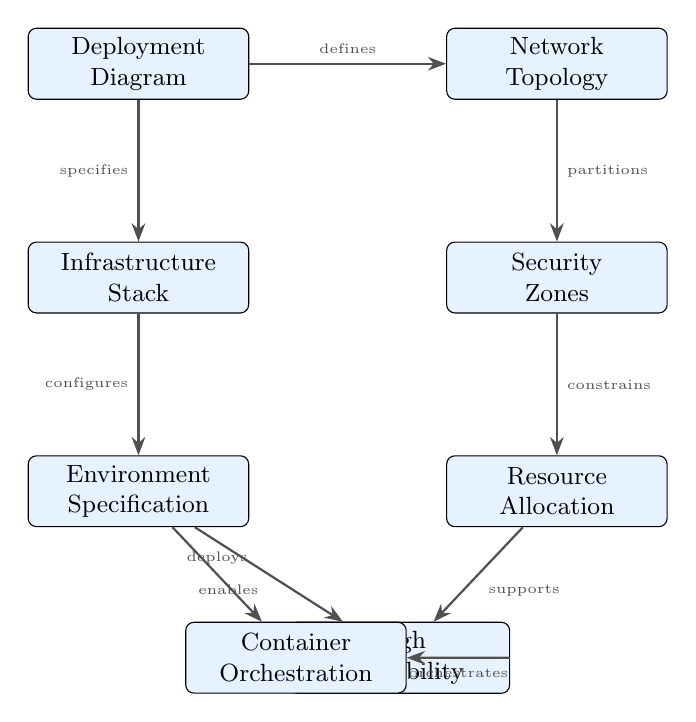
\begin{tikzpicture}[
    node distance=1.8cm and 2.5cm,
    model/.style={draw, fill=nodecolor, rounded corners=3pt, minimum width=2.8cm, minimum height=0.9cm, font=\small, align=center},
    arrow/.style={-{Stealth}, thick, darkgray}
]
    % Nodes
    \node[model] (deploy) {Deployment\\Diagram};
    \node[model, right=of deploy] (network) {Network\\Topology};
    \node[model, below=of deploy] (stack) {Infrastructure\\Stack};
    \node[model, below=of network] (security) {Security\\Zones};
    \node[model, below=of stack] (env) {Environment\\Specification};
    \node[model, below=of security] (resource) {Resource\\Allocation};
    \node[model, below right=1.2cm and 0.5cm of env] (ha) {High\\Availability};
    \node[model, below left=1.2cm and 0.5cm of resource] (container) {Container\\Orchestration};
    
    % Arrows
    \draw[arrow] (deploy) -- (network) node[midway, above, font=\tiny] {defines};
    \draw[arrow] (deploy) -- (stack) node[midway, left, font=\tiny] {specifies};
    \draw[arrow] (network) -- (security) node[midway, right, font=\tiny] {partitions};
    \draw[arrow] (stack) -- (env) node[midway, left, font=\tiny] {configures};
    \draw[arrow] (security) -- (resource) node[midway, right, font=\tiny] {constrains};
    \draw[arrow] (env) -- (ha) node[midway, below left, font=\tiny] {enables};
    \draw[arrow] (resource) -- (ha) node[midway, below right, font=\tiny] {supports};
    \draw[arrow] (env) -- (container) node[midway, above, font=\tiny] {deploys};
    \draw[arrow] (ha) -- (container) node[midway, below, font=\tiny] {orchestrates};
\end{tikzpicture}
\caption{Model Type Dependency Relationships}
\end{figure}

% =============================================================================
% SECTION: MODEL LANGUAGES
% =============================================================================
\section{Model Languages}

For each model type, specific languages, notations, and modeling techniques are prescribed. This section documents the vocabulary and grammar for constructing deployment views.

\subsection{UML Deployment Diagram Notation}

The Unified Modeling Language (UML) provides a standardized notation for deployment diagrams that is widely recognized and tool-supported.

\subsubsection{Primary Notation Elements}

\begin{table}[H]
\centering
\caption{UML Deployment Diagram Notation Elements}
\small
\begin{tabular}{@{}C{3cm}L{4cm}L{6.5cm}@{}}
\toprule
\textbf{Symbol} & \textbf{Element} & \textbf{Description} \\
\midrule
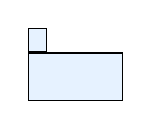
\begin{tikzpicture}[baseline=-0.5ex]
    \node[draw, fill=nodecolor, minimum width=1.2cm, minimum height=0.6cm] (n) {};
    \node[draw, fill=nodecolor, minimum width=0.15cm, minimum height=0.3cm, anchor=south west] at (n.north west) {};
\end{tikzpicture} & Node & Physical or virtual computing resource capable of hosting software \\
\addlinespace
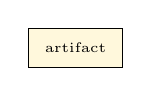
\begin{tikzpicture}[baseline=-0.5ex]
    \node[draw, fill=componentcolor, minimum width=1.2cm, minimum height=0.5cm] (a) {};
    \node[font=\tiny] at (a.center) {artifact};
\end{tikzpicture} & Artifact & Deployable software element (executable, library, configuration) \\
\addlinespace
\begin{tikzpicture}[baseline=-0.5ex]
    \draw[thick] (0,0) -- (1,0);
\end{tikzpicture} & Association & General relationship between elements \\
\addlinespace
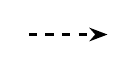
\begin{tikzpicture}[baseline=-0.5ex]
    \draw[thick, dashed, -{Stealth}] (0,0) -- (1,0);
\end{tikzpicture} & Dependency & One element depends on another \\
\addlinespace
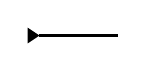
\begin{tikzpicture}[baseline=-0.5ex]
    \draw[thick] (0,0) -- (1,0);
    \fill (0,0) -- (-0.15,0.1) -- (-0.15,-0.1) -- cycle;
\end{tikzpicture} & Composition & Strong ownership relationship \\
\bottomrule
\end{tabular}
\end{table}

\subsubsection{Node Stereotypes}

UML stereotypes extend the base notation to represent specific infrastructure types:

\begin{table}[H]
\centering
\caption{Common Node Stereotypes}
\small
\begin{tabular}{@{}L{3.5cm}L{10cm}@{}}
\toprule
\textbf{Stereotype} & \textbf{Description} \\
\midrule
\texttt{<<device>>} & Physical hardware device \\
\texttt{<<executionEnvironment>>} & Runtime environment (JVM, container, etc.) \\
\texttt{<<server>>} & Server machine (physical or virtual) \\
\texttt{<<database>>} & Database server or instance \\
\texttt{<<container>>} & Container runtime (Docker, etc.) \\
\texttt{<<pod>>} & Kubernetes pod \\
\texttt{<<cluster>>} & Cluster of nodes \\
\texttt{<<loadBalancer>>} & Load balancing device or service \\
\texttt{<<firewall>>} & Network firewall \\
\texttt{<<storage>>} & Storage system or volume \\
\texttt{<<cloud>>} & Cloud infrastructure service \\
\bottomrule
\end{tabular}
\end{table}

\subsection{Network Diagram Notation}

Network topology diagrams employ industry-standard symbols and conventions for representing infrastructure.

\begin{figure}[H]
\centering
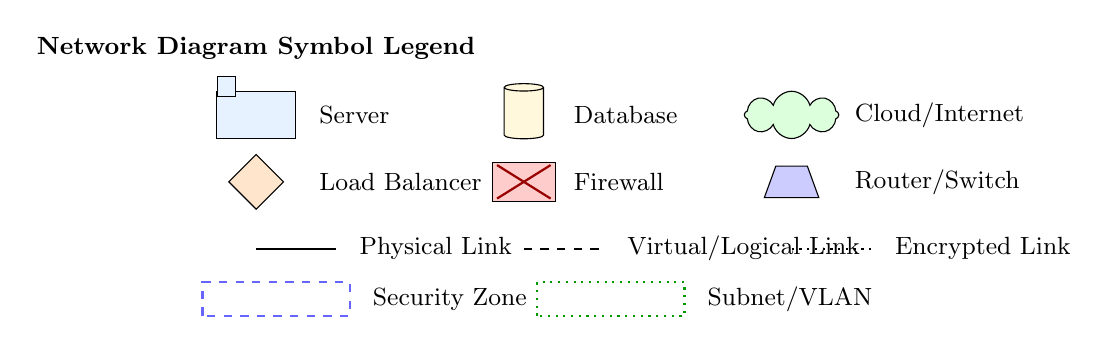
\begin{tikzpicture}[scale=0.85]
    % Legend items
    \node[font=\small\bfseries] at (0, 4) {Network Diagram Symbol Legend};
    
    % Row 1
    \node[draw, fill=nodecolor, minimum width=1cm, minimum height=0.6cm] at (0, 3) {};
    \node[draw, fill=nodecolor, minimum width=0.12cm, minimum height=0.25cm] at (-0.44, 3.42) {};
    \node[right, font=\small] at (0.8, 3) {Server};
    
    \node[draw, fill=componentcolor, cylinder, shape border rotate=90, aspect=0.4, minimum height=0.7cm, minimum width=0.5cm] at (4, 3) {};
    \node[right, font=\small] at (4.6, 3) {Database};
    
    \node[draw, fill=connectorcolor, cloud, cloud puffs=8, minimum width=1.2cm, minimum height=0.6cm, inner sep=0pt] at (8, 3) {};
    \node[right, font=\small] at (8.8, 3) {Cloud/Internet};
    
    % Row 2
    \node[draw, fill=orange!20, diamond, minimum width=0.7cm, minimum height=0.7cm] at (0, 2) {};
    \node[right, font=\small] at (0.8, 2) {Load Balancer};
    
    \node[draw, fill=red!20, rectangle, minimum width=0.8cm, minimum height=0.5cm] at (4, 2) {};
    \draw[thick, red!60!black] (3.6, 1.75) -- (4.4, 2.25);
    \draw[thick, red!60!black] (3.6, 2.25) -- (4.4, 1.75);
    \node[right, font=\small] at (4.6, 2) {Firewall};
    
    \node[draw, fill=blue!20, trapezium, trapezium angle=70, minimum width=0.6cm, minimum height=0.4cm] at (8, 2) {};
    \node[right, font=\small] at (8.8, 2) {Router/Switch};
    
    % Row 3 - Line types
    \draw[thick] (0, 1) -- (1.2, 1);
    \node[right, font=\small] at (1.4, 1) {Physical Link};
    
    \draw[thick, dashed] (4, 1) -- (5.2, 1);
    \node[right, font=\small] at (5.4, 1) {Virtual/Logical Link};
    
    \draw[thick, dotted] (8, 1) -- (9.2, 1);
    \node[right, font=\small] at (9.4, 1) {Encrypted Link};
    
    % Row 4 - Zones
    \draw[thick, dashed, blue!60] (-0.8, 0) rectangle (1.4, 0.5);
    \node[right, font=\small] at (1.6, 0.25) {Security Zone};
    
    \draw[thick, dotted, green!60!black] (4.2, 0) rectangle (6.4, 0.5);
    \node[right, font=\small] at (6.6, 0.25) {Subnet/VLAN};
\end{tikzpicture}
\caption{Network Diagram Symbol Legend}
\end{figure}

\subsection{Infrastructure as Code Languages}

Modern deployment documentation often includes or references Infrastructure as Code (IaC) specifications. The following languages are commonly used:

\begin{table}[H]
\centering
\caption{Infrastructure as Code Languages}
\small
\begin{tabular}{@{}L{2.5cm}L{3cm}L{8cm}@{}}
\toprule
\textbf{Language} & \textbf{Platform} & \textbf{Use Case} \\
\midrule
Terraform HCL & Multi-cloud & Declarative infrastructure provisioning across cloud providers \\
CloudFormation & AWS & AWS-native infrastructure definition \\
ARM Templates & Azure & Azure resource deployment specifications \\
Kubernetes YAML & Container orchestration & Container workload definitions and configurations \\
Docker Compose & Container deployment & Multi-container application definitions \\
Ansible YAML & Configuration management & Server configuration and application deployment \\
Pulumi & Multi-cloud & Programmatic infrastructure using general-purpose languages \\
\bottomrule
\end{tabular}
\end{table}

\subsection{Tabular Specifications}

Many deployment details are best captured in tabular form. Standard table formats include:

\subsubsection{Node Specification Table}

\begin{table}[H]
\centering
\caption{Example Node Specification Table Format}
\small
\begin{tabular}{@{}L{2cm}L{2cm}L{1.5cm}L{1.5cm}L{1.5cm}L{1.8cm}L{2cm}@{}}
\toprule
\textbf{Node ID} & \textbf{Type} & \textbf{vCPU} & \textbf{RAM} & \textbf{Storage} & \textbf{OS} & \textbf{Purpose} \\
\midrule
web-01 & VM & 4 & 16 GB & 100 GB & Ubuntu 22.04 & Web Server \\
app-01 & VM & 8 & 32 GB & 200 GB & Ubuntu 22.04 & App Server \\
db-01 & VM & 16 & 64 GB & 1 TB & Ubuntu 22.04 & Primary DB \\
\bottomrule
\end{tabular}
\end{table}

\subsubsection{Network Connection Table}

\begin{table}[H]
\centering
\caption{Example Network Connection Table Format}
\small
\begin{tabular}{@{}L{2cm}L{2cm}L{2cm}L{2cm}L{2cm}L{2.5cm}@{}}
\toprule
\textbf{Source} & \textbf{Target} & \textbf{Protocol} & \textbf{Port(s)} & \textbf{Direction} & \textbf{Purpose} \\
\midrule
web-01 & app-01 & HTTPS & 443 & Outbound & API calls \\
app-01 & db-01 & PostgreSQL & 5432 & Outbound & Database queries \\
lb-01 & web-* & HTTP/S & 80, 443 & Outbound & Load distribution \\
\bottomrule
\end{tabular}
\end{table}

% =============================================================================
% SECTION: VIEWPOINT METAMODELS
% =============================================================================
\section{Viewpoint Metamodels}

This section defines the conceptual metamodel underlying the Deployment Viewpoint. The metamodel establishes the vocabulary of element types, their properties, and valid relationships.

\subsection{Core Metamodel}

\begin{figure}[H]
\centering
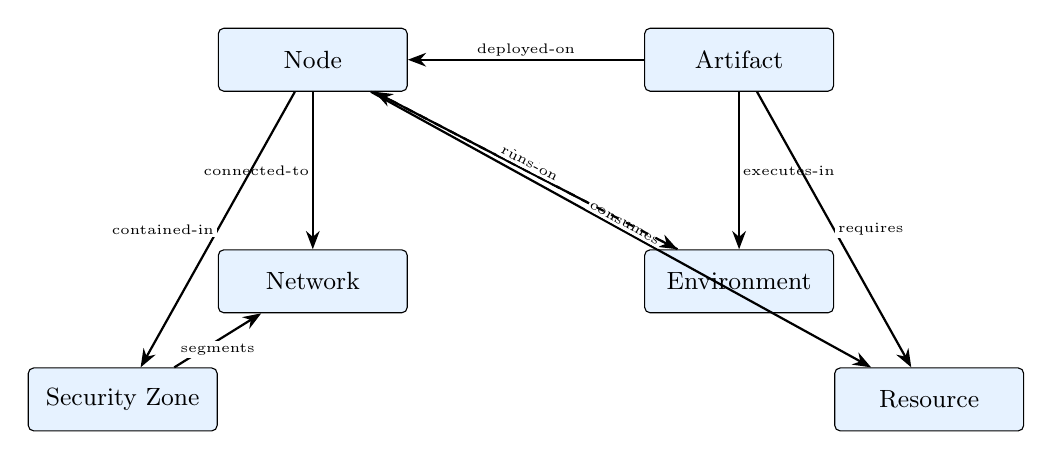
\begin{tikzpicture}[
    node distance=1.5cm and 2.5cm,
    entity/.style={draw, fill=nodecolor, rounded corners=2pt, minimum width=2.4cm, minimum height=0.8cm, font=\small},
    relation/.style={draw, fill=componentcolor, diamond, minimum width=1.8cm, minimum height=0.6cm, font=\tiny},
    arrow/.style={-{Stealth}, thick},
    label/.style={font=\tiny, fill=white, inner sep=1pt}
]
    % Main entities
    \node[entity] (node) {Node};
    \node[entity, right=3cm of node] (artifact) {Artifact};
    \node[entity, below=2cm of node] (network) {Network};
    \node[entity, below=2cm of artifact] (env) {Environment};
    \node[entity, below left=3.5cm and 0cm of node] (zone) {Security Zone};
    \node[entity, below right=3.5cm and 0cm of artifact] (resource) {Resource};
    
    % Relationships
    \draw[arrow] (artifact) -- (node) node[label, midway, above] {deployed-on};
    \draw[arrow] (node) -- (network) node[label, midway, left] {connected-to};
    \draw[arrow] (node) -- (env) node[label, midway, above, sloped] {hosts};
    \draw[arrow] (artifact) -- (env) node[label, midway, right] {executes-in};
    \draw[arrow] (node) -- (zone) node[label, midway, left] {contained-in};
    \draw[arrow] (node) -- (resource) node[label, midway, above, sloped] {consumes};
    \draw[arrow] (artifact) -- (resource) node[label, midway, right] {requires};
    \draw[arrow] (zone) -- (network) node[label, midway, below] {segments};
    
    % Inheritance relationships
    \draw[arrow, dashed] (env) -- (node) node[label, midway, above, sloped] {runs-on};
\end{tikzpicture}
\caption{Deployment Viewpoint Core Metamodel}
\end{figure}

\subsection{Entity Definitions}

\begin{definitionbox}[Entity: Node]
\textbf{Definition:} A computational resource capable of hosting and executing software artifacts.

\textbf{Attributes:}
\begin{itemize}[nosep]
    \item \texttt{nodeId}: Unique identifier for the node
    \item \texttt{name}: Human-readable name
    \item \texttt{type}: Classification (physical, virtual, container, serverless)
    \item \texttt{hostname}: Network hostname
    \item \texttt{ipAddresses}: List of IP addresses
    \item \texttt{operatingSystem}: OS type and version
    \item \texttt{status}: Operational status (active, standby, maintenance)
    \item \texttt{location}: Physical or logical location
    \item \texttt{provider}: Infrastructure provider (on-premise, AWS, Azure, GCP)
\end{itemize}

\textbf{Constraints:}
\begin{itemize}[nosep]
    \item Each node must have a unique \texttt{nodeId}
    \item Virtual nodes must reference a parent physical node or hypervisor
    \item Container nodes must reference a container runtime environment
\end{itemize}
\end{definitionbox}

\begin{definitionbox}[Entity: Artifact]
\textbf{Definition:} A deployable unit of software that can be installed on and executed by a node.

\textbf{Attributes:}
\begin{itemize}[nosep]
    \item \texttt{artifactId}: Unique identifier
    \item \texttt{name}: Artifact name
    \item \texttt{version}: Version identifier
    \item \texttt{type}: Artifact type (executable, library, container image, configuration)
    \item \texttt{checksum}: Integrity verification hash
    \item \texttt{size}: Artifact size in bytes
    \item \texttt{repository}: Source repository location
    \item \texttt{buildInfo}: Build metadata (commit, timestamp, builder)
\end{itemize}

\textbf{Constraints:}
\begin{itemize}[nosep]
    \item Artifact version must follow semantic versioning
    \item Container images must include registry and tag information
    \item Configuration artifacts must specify target environment
\end{itemize}
\end{definitionbox}

\begin{definitionbox}[Entity: Network]
\textbf{Definition:} A communication infrastructure that connects nodes and enables data exchange.

\textbf{Attributes:}
\begin{itemize}[nosep]
    \item \texttt{networkId}: Unique identifier
    \item \texttt{name}: Network name
    \item \texttt{type}: Network type (LAN, WAN, VPC, overlay)
    \item \texttt{cidrBlock}: IP address range
    \item \texttt{vlanId}: VLAN identifier (if applicable)
    \item \texttt{mtu}: Maximum transmission unit
    \item \texttt{bandwidth}: Available bandwidth
    \item \texttt{latency}: Expected latency characteristics
\end{itemize}

\textbf{Constraints:}
\begin{itemize}[nosep]
    \item CIDR blocks must not overlap within the same network domain
    \item Connected nodes must have compatible network configurations
\end{itemize}
\end{definitionbox}

\begin{definitionbox}[Entity: Environment]
\textbf{Definition:} A runtime context that provides services and resources for artifact execution.

\textbf{Attributes:}
\begin{itemize}[nosep]
    \item \texttt{environmentId}: Unique identifier
    \item \texttt{name}: Environment name (e.g., production, staging, development)
    \item \texttt{type}: Environment type (bare metal, VM, container, serverless)
    \item \texttt{runtime}: Runtime platform (JVM, Node.js, Python, .NET)
    \item \texttt{runtimeVersion}: Runtime version
    \item \texttt{configuration}: Environment-specific configuration
    \item \texttt{variables}: Environment variables
\end{itemize}

\textbf{Constraints:}
\begin{itemize}[nosep]
    \item Environment configurations must be complete for artifact execution
    \item Sensitive configuration values must be stored securely
\end{itemize}
\end{definitionbox}

\begin{definitionbox}[Entity: Security Zone]
\textbf{Definition:} A logical boundary that groups nodes with similar security requirements and trust levels.

\textbf{Attributes:}
\begin{itemize}[nosep]
    \item \texttt{zoneId}: Unique identifier
    \item \texttt{name}: Zone name (e.g., DMZ, internal, restricted)
    \item \texttt{trustLevel}: Security classification level
    \item \texttt{accessPolicy}: Default access control policy
    \item \texttt{encryptionRequired}: Whether encryption is mandated
    \item \texttt{complianceRequirements}: Applicable compliance standards
\end{itemize}

\textbf{Constraints:}
\begin{itemize}[nosep]
    \item Cross-zone communication must traverse security controls
    \item Higher trust zones cannot directly access lower trust zones
\end{itemize}
\end{definitionbox}

\begin{definitionbox}[Entity: Resource]
\textbf{Definition:} A computational, storage, or network resource that can be allocated to nodes or artifacts.

\textbf{Attributes:}
\begin{itemize}[nosep]
    \item \texttt{resourceId}: Unique identifier
    \item \texttt{type}: Resource type (CPU, memory, storage, network bandwidth)
    \item \texttt{capacity}: Total available capacity
    \item \texttt{allocated}: Currently allocated amount
    \item \texttt{unit}: Unit of measurement
    \item \texttt{sharable}: Whether resource can be shared
    \item \texttt{elasticity}: Auto-scaling capability
\end{itemize}

\textbf{Constraints:}
\begin{itemize}[nosep]
    \item Allocated resources cannot exceed capacity
    \item Resource reservations must be honored by schedulers
\end{itemize}
\end{definitionbox}

\subsection{Relationship Definitions}

\begin{table}[H]
\centering
\caption{Metamodel Relationship Definitions}
\small
\begin{tabular}{@{}L{2.8cm}L{2cm}L{2cm}L{6.5cm}@{}}
\toprule
\textbf{Relationship} & \textbf{Source} & \textbf{Target} & \textbf{Description} \\
\midrule
deployed-on & Artifact & Node & Artifact is installed and runs on the node \\
\addlinespace
connected-to & Node & Network & Node has network connectivity through this network \\
\addlinespace
hosts & Node & Environment & Node provides the environment for execution \\
\addlinespace
executes-in & Artifact & Environment & Artifact runs within this execution environment \\
\addlinespace
contained-in & Node & Security Zone & Node is located within this security boundary \\
\addlinespace
consumes & Node & Resource & Node uses this resource for operation \\
\addlinespace
requires & Artifact & Resource & Artifact needs this resource to function \\
\addlinespace
segments & Security Zone & Network & Zone defines a partition of the network \\
\addlinespace
communicates-with & Node & Node & Direct communication path between nodes \\
\addlinespace
replicates & Node & Node & Data or state replication relationship \\
\addlinespace
fails-over-to & Node & Node & Failover target in case of primary failure \\
\addlinespace
load-balances & Node & Node & Traffic distribution relationship \\
\bottomrule
\end{tabular}
\end{table}

% =============================================================================
% SECTION: CONFORMING NOTATIONS
% =============================================================================
\section{Conforming Notations}

Several existing notations and modeling languages conform to the Deployment Viewpoint metamodel and may be used interchangeably or in combination.

\subsection{UML 2.x Deployment Diagrams}

The UML 2.x specification defines deployment diagrams as a standard notation for showing the physical arrangement of artifacts on nodes. UML deployment diagrams provide native support for nodes, artifacts, communication paths, and deployment specifications.

\textbf{Conformance Level:} Full conformance to core metamodel elements.

\textbf{Tool Support:} Enterprise Architect, Visual Paradigm, StarUML, PlantUML, Lucidchart, draw.io.

\subsection{C4 Model - Deployment Diagram}

The C4 model includes a deployment diagram type that shows how software systems and containers are deployed onto infrastructure. C4 deployment diagrams emphasize clarity and audience-appropriate abstraction levels.

\textbf{Conformance Level:} Partial conformance; focuses on container-level deployment rather than fine-grained artifacts.

\textbf{Tool Support:} Structurizr, PlantUML (C4 extension), IcePanel.

\subsection{ArchiMate Technology Layer}

ArchiMate's Technology Layer provides notation for modeling infrastructure elements including nodes, devices, system software, networks, and communication paths.

\textbf{Conformance Level:} Full conformance with extended enterprise architecture context.

\textbf{Tool Support:} Archi, BiZZdesign, MEGA, Sparx Enterprise Architect.

\subsection{AWS/Azure/GCP Architecture Diagrams}

Cloud providers offer official icon sets and diagram conventions for documenting cloud infrastructure deployments.

\textbf{Conformance Level:} Platform-specific conformance with rich service representation.

\textbf{Tool Support:} AWS Architecture Icons, Azure Architecture Icons, Google Cloud Architecture Diagramming Tool, Cloudcraft, Lucidchart, draw.io.

\subsection{Kubernetes Architecture Diagrams}

For containerized deployments, Kubernetes-specific notation captures clusters, nodes, pods, services, and networking constructs.

\textbf{Conformance Level:} Container orchestration-specific conformance.

\textbf{Tool Support:} Lens, k8sviz, KubeView, custom tooling.

\begin{table}[H]
\centering
\caption{Notation Comparison Matrix}
\footnotesize
\begin{tabular}{@{}L{2.5cm}C{1.3cm}C{1.3cm}C{1.3cm}C{1.3cm}C{1.3cm}C{1.3cm}@{}}
\toprule
\textbf{Feature} & \rotatebox{60}{\textbf{UML 2.x}} & \rotatebox{60}{\textbf{C4 Model}} & \rotatebox{60}{\textbf{ArchiMate}} & \rotatebox{60}{\textbf{Cloud Icons}} & \rotatebox{60}{\textbf{K8s Native}} & \rotatebox{60}{\textbf{Custom}} \\
\midrule
Physical Nodes & $\bullet$ & $\bullet$ & $\bullet$ & $\bullet$ & $\circ$ & $\bullet$ \\
Virtual Machines & $\bullet$ & $\bullet$ & $\bullet$ & $\bullet$ & $\circ$ & $\bullet$ \\
Containers & $\circ$ & $\bullet$ & $\circ$ & $\bullet$ & $\bullet$ & $\bullet$ \\
Networks & $\bullet$ & $\circ$ & $\bullet$ & $\bullet$ & $\bullet$ & $\bullet$ \\
Security Zones & $\circ$ & $\circ$ & $\bullet$ & $\bullet$ & $\circ$ & $\bullet$ \\
Cloud Services & $\circ$ & $\circ$ & $\circ$ & $\bullet$ & $\circ$ & $\bullet$ \\
Standardized & $\bullet$ & $\bullet$ & $\bullet$ & $\circ$ & $\circ$ & -- \\
Tool Support & $\bullet$ & $\bullet$ & $\bullet$ & $\bullet$ & $\circ$ & $\circ$ \\
\bottomrule
\multicolumn{7}{l}{\footnotesize $\bullet$ = Strong support, $\circ$ = Limited support, -- = Not applicable}
\end{tabular}
\end{table}

% =============================================================================
% SECTION: MODEL CORRESPONDENCE RULES
% =============================================================================
\section{Model Correspondence Rules}

Model correspondence rules define how elements in deployment models relate to elements in other architectural views. These rules ensure consistency across the architecture documentation.

\subsection{Component-and-Connector View Correspondence}

\begin{definitionbox}[Correspondence Rule CR-01: Component to Artifact Mapping]
\textbf{Rule:} Every runtime component identified in a Component-and-Connector view must correspond to one or more deployment artifacts.

\textbf{Formal Expression:}
\begin{center}
$\forall c \in Components_{C\&C} : \exists a \in Artifacts_{Deploy} : manifests(a, c)$
\end{center}

\textbf{Rationale:} Ensures that all software components have a concrete deployment representation.

\textbf{Verification:} Traceability matrix linking components to artifacts.
\end{definitionbox}

\begin{definitionbox}[Correspondence Rule CR-02: Connector to Network Path Mapping]
\textbf{Rule:} Every connector between components in a C\&C view that crosses node boundaries must have a corresponding network path in the deployment model.

\textbf{Formal Expression:}
\begin{center}
$\forall conn(c_1, c_2) : node(c_1) \neq node(c_2) \Rightarrow \exists path(node(c_1), node(c_2))$
\end{center}

\textbf{Rationale:} Validates that required communication paths exist in the infrastructure.

\textbf{Verification:} Network connectivity analysis.
\end{definitionbox}

\subsection{Module View Correspondence}

\begin{definitionbox}[Correspondence Rule CR-03: Module to Artifact Packaging]
\textbf{Rule:} The module decomposition structure should be reflected in artifact packaging boundaries.

\textbf{Formal Expression:}
\begin{center}
$\forall m \in Modules : packaged\_in(m) \subseteq Artifacts$
\end{center}

\textbf{Rationale:} Maintains alignment between logical module structure and physical deployment units.

\textbf{Verification:} Build manifest analysis.
\end{definitionbox}

\subsection{Data View Correspondence}

\begin{definitionbox}[Correspondence Rule CR-04: Data Store to Storage Node Mapping]
\textbf{Rule:} Every persistent data store identified in a data architecture view must be allocated to storage infrastructure in the deployment model.

\textbf{Formal Expression:}
\begin{center}
$\forall ds \in DataStores : \exists n \in Nodes : hosts(n, ds) \land type(n) = storage$
\end{center}

\textbf{Rationale:} Ensures all data has defined storage infrastructure.

\textbf{Verification:} Data residency mapping.
\end{definitionbox}

\subsection{Security View Correspondence}

\begin{definitionbox}[Correspondence Rule CR-05: Trust Boundary to Security Zone Mapping]
\textbf{Rule:} Trust boundaries defined in security architecture must align with security zone definitions in the deployment model.

\textbf{Formal Expression:}
\begin{center}
$\forall tb \in TrustBoundaries : \exists sz \in SecurityZones : implements(sz, tb)$
\end{center}

\textbf{Rationale:} Validates that security architecture is realized in deployment.

\textbf{Verification:} Security zone audit.
\end{definitionbox}

\subsection{Correspondence Verification Matrix}

\begin{table}[H]
\centering
\caption{Cross-View Correspondence Verification}
\small
\begin{tabular}{@{}L{2.5cm}L{3.5cm}L{3.5cm}L{3.5cm}@{}}
\toprule
\textbf{Rule ID} & \textbf{Source View} & \textbf{Target Elements} & \textbf{Verification Method} \\
\midrule
CR-01 & C\&C Components & Deployment Artifacts & Traceability matrix \\
CR-02 & C\&C Connectors & Network Paths & Connectivity analysis \\
CR-03 & Module Structure & Artifact Packages & Build manifest review \\
CR-04 & Data Stores & Storage Nodes & Data residency mapping \\
CR-05 & Trust Boundaries & Security Zones & Security zone audit \\
\bottomrule
\end{tabular}
\end{table}

% =============================================================================
% SECTION: OPERATIONS ON VIEWS
% =============================================================================
\section{Operations on Views}

This section defines the methods and procedures for creating, interpreting, analyzing, and implementing deployment views.

\subsection{Creation Methods}

\subsubsection{View Development Process}

\begin{guidancebox}[Step 1: Establish Scope and Context]
\begin{enumerate}[nosep]
    \item Identify the system or subsystem to be documented
    \item Determine the deployment scenarios (development, staging, production)
    \item Identify target infrastructure platforms
    \item Gather existing infrastructure documentation
    \item Interview key stakeholders (operations, security, development)
\end{enumerate}
\end{guidancebox}

\begin{guidancebox}[Step 2: Identify Deployment Elements]
\begin{enumerate}[nosep]
    \item List all deployable software artifacts from Component-and-Connector views
    \item Identify required runtime environments and dependencies
    \item Document hardware and virtual infrastructure nodes
    \item Map network topology and connectivity requirements
    \item Define security zones and trust boundaries
\end{enumerate}
\end{guidancebox}

\begin{guidancebox}[Step 3: Create Initial Deployment Model]
\begin{enumerate}[nosep]
    \item Draw high-level deployment topology showing major nodes
    \item Allocate software artifacts to execution nodes
    \item Define network connections and communication paths
    \item Overlay security zone boundaries
    \item Document resource allocations and constraints
\end{enumerate}
\end{guidancebox}

\begin{guidancebox}[Step 4: Elaborate and Refine]
\begin{enumerate}[nosep]
    \item Add detailed node specifications (hardware, OS, middleware)
    \item Document environment-specific configurations
    \item Specify high availability and redundancy mechanisms
    \item Define scaling policies and capacity limits
    \item Add monitoring and observability infrastructure
\end{enumerate}
\end{guidancebox}

\begin{guidancebox}[Step 5: Validate and Review]
\begin{enumerate}[nosep]
    \item Verify correspondence with other architectural views
    \item Validate against quality attribute requirements
    \item Review with infrastructure and security teams
    \item Conduct deployment feasibility assessment
    \item Document decisions, rationale, and trade-offs
\end{enumerate}
\end{guidancebox}

\subsubsection{Documentation Templates}

\textbf{Node Documentation Template:}

\begin{lstlisting}[caption={Node Specification Template}]
Node Specification
==================
Node ID:        [Unique identifier]
Name:           [Human-readable name]
Type:           [Physical | Virtual | Container | Serverless]
Purpose:        [Primary function and role]

Hardware/Resources:
  - CPU:        [Cores/vCPUs and type]
  - Memory:     [RAM capacity]
  - Storage:    [Disk capacity and type]
  - Network:    [Network interfaces]

Software Stack:
  - OS:         [Operating system and version]
  - Runtime:    [Runtime environments]
  - Middleware: [Middleware components]

Network Configuration:
  - Hostname:   [FQDN]
  - IP Address: [Static IP or DHCP]
  - DNS:        [DNS entries]
  - Ports:      [Open ports and protocols]

Deployed Artifacts:
  - [List of deployed software components]

Dependencies:
  - [External service dependencies]

Notes:
  - [Additional configuration notes]
\end{lstlisting}

\subsubsection{Common Patterns and Idioms}

\begin{table}[H]
\centering
\caption{Deployment Patterns}
\small
\begin{tabular}{@{}L{3cm}L{5cm}L{5.5cm}@{}}
\toprule
\textbf{Pattern} & \textbf{Description} & \textbf{Use When} \\
\midrule
Single Server & All components on one node & Development, small-scale applications \\
\addlinespace
N-Tier & Separate tiers for web, app, data & Traditional enterprise applications \\
\addlinespace
Microservices & Independent service deployment & Scalable, independently deployable services \\
\addlinespace
Container Cluster & Orchestrated container deployment & Cloud-native, dynamic scaling needs \\
\addlinespace
Serverless & Function-based deployment & Event-driven, variable workloads \\
\addlinespace
Hybrid Cloud & Mix of on-premise and cloud & Data sovereignty, burst capacity \\
\addlinespace
Multi-Region & Geographic distribution & High availability, low latency globally \\
\addlinespace
Blue-Green & Parallel production environments & Zero-downtime deployments \\
\addlinespace
Canary & Gradual traffic shifting & Risk mitigation for new releases \\
\bottomrule
\end{tabular}
\end{table}

\subsection{Interpretive Methods}

\subsubsection{Reading Deployment Diagrams}

When interpreting a deployment view, stakeholders should follow this systematic approach:

\begin{enumerate}
    \item \textbf{Identify the Scope:} Determine what system or subsystem is depicted and for which environment(s).
    
    \item \textbf{Understand Node Types:} Distinguish between physical servers, virtual machines, containers, and cloud services based on notation and stereotypes.
    
    \item \textbf{Trace Software Allocation:} For each software component of interest, identify which node(s) host it and in what configuration.
    
    \item \textbf{Analyze Connectivity:} Follow communication paths between nodes, noting protocols, ports, and any intermediate network devices.
    
    \item \textbf{Identify Security Boundaries:} Locate security zone boundaries and understand the trust levels and access controls between zones.
    
    \item \textbf{Assess Redundancy:} Look for redundant nodes, load balancers, and failover paths that support availability requirements.
    
    \item \textbf{Check Resource Allocations:} Review resource specifications to understand capacity and potential constraints.
\end{enumerate}

\subsubsection{Stakeholder-Specific Interpretation Guides}

\textbf{For System Administrators:}
Focus on node specifications, installed software, network configurations, and operational procedures. Pay attention to monitoring integration points and log aggregation paths.

\textbf{For Security Teams:}
Prioritize security zone boundaries, network segmentation, encryption points, and access control mechanisms. Validate that sensitive components are appropriately isolated.

\textbf{For Development Teams:}
Understand the runtime environments available, deployed artifact versions, configuration management approaches, and paths from development to production.

\textbf{For Capacity Planners:}
Examine resource allocations, scaling policies, current utilization levels, and growth projections. Identify potential bottlenecks and scaling limits.

\subsection{Analysis Methods}

\subsubsection{Performance Analysis}

\begin{definitionbox}[Performance Analysis Technique]
\textbf{Purpose:} Evaluate whether the deployment topology can meet performance requirements.

\textbf{Inputs:}
\begin{itemize}[nosep]
    \item Deployment model with resource specifications
    \item Performance requirements (response time, throughput)
    \item Workload characteristics (request rates, data volumes)
\end{itemize}

\textbf{Process:}
\begin{enumerate}[nosep]
    \item Model system as a queuing network
    \item Assign service rates based on resource specifications
    \item Apply workload arrival rates
    \item Calculate utilization, queue lengths, and response times
    \item Compare against requirements
\end{enumerate}

\textbf{Outputs:}
\begin{itemize}[nosep]
    \item Predicted performance metrics
    \item Identified bottlenecks
    \item Scaling recommendations
\end{itemize}
\end{definitionbox}

\subsubsection{Availability Analysis}

\begin{definitionbox}[Availability Analysis Technique]
\textbf{Purpose:} Calculate expected system availability based on deployment redundancy.

\textbf{Inputs:}
\begin{itemize}[nosep]
    \item Deployment topology with redundancy configuration
    \item Component reliability data (MTBF, MTTR)
    \item Failover mechanisms and recovery times
\end{itemize}

\textbf{Process:}
\begin{enumerate}[nosep]
    \item Construct reliability block diagram from deployment
    \item Identify serial and parallel configurations
    \item Calculate composite availability using formulas:
    \begin{itemize}[nosep]
        \item Serial: $A_{total} = A_1 \times A_2 \times ... \times A_n$
        \item Parallel: $A_{total} = 1 - (1-A_1) \times (1-A_2) \times ... \times (1-A_n)$
    \end{itemize}
    \item Account for failover time impacts
    \item Compare against availability targets
\end{enumerate}

\textbf{Outputs:}
\begin{itemize}[nosep]
    \item Predicted availability percentage
    \item Single points of failure identification
    \item Redundancy improvement recommendations
\end{itemize}
\end{definitionbox}

\subsubsection{Security Analysis}

\begin{definitionbox}[Security Posture Analysis Technique]
\textbf{Purpose:} Evaluate the security effectiveness of the deployment architecture.

\textbf{Inputs:}
\begin{itemize}[nosep]
    \item Deployment model with security zones
    \item Network segmentation configuration
    \item Access control policies
    \item Threat model and attack vectors
\end{itemize}

\textbf{Process:}
\begin{enumerate}[nosep]
    \item Map attack surface from external entry points
    \item Trace potential attack paths through the deployment
    \item Evaluate defense-in-depth layers
    \item Assess data protection at rest and in transit
    \item Review compliance against security requirements
\end{enumerate}

\textbf{Outputs:}
\begin{itemize}[nosep]
    \item Security risk assessment
    \item Vulnerability identification
    \item Hardening recommendations
\end{itemize}
\end{definitionbox}

\subsubsection{Cost Analysis}

\begin{definitionbox}[Total Cost of Ownership Analysis]
\textbf{Purpose:} Estimate the total cost of the deployment configuration.

\textbf{Inputs:}
\begin{itemize}[nosep]
    \item Deployment model with all resources
    \item Pricing information (hardware, cloud, licensing)
    \item Operational cost factors
    \item Time horizon for analysis
\end{itemize}

\textbf{Process:}
\begin{enumerate}[nosep]
    \item Calculate infrastructure costs (compute, storage, network)
    \item Add software licensing costs
    \item Estimate operational costs (personnel, support)
    \item Project costs over analysis period
    \item Compare alternatives if applicable
\end{enumerate}

\textbf{Outputs:}
\begin{itemize}[nosep]
    \item Total cost estimate
    \item Cost breakdown by category
    \item Cost optimization opportunities
\end{itemize}
\end{definitionbox}

\subsection{Implementation Methods}

\subsubsection{Deployment Automation}

Modern deployment implementation relies heavily on automation. The deployment view serves as the specification for Infrastructure as Code implementations.

\begin{table}[H]
\centering
\caption{Implementation Automation Approaches}
\small
\begin{tabular}{@{}L{3cm}L{4.5cm}L{6cm}@{}}
\toprule
\textbf{Approach} & \textbf{Tools} & \textbf{Description} \\
\midrule
Infrastructure Provisioning & Terraform, CloudFormation, Pulumi & Declaratively provision cloud and on-premise infrastructure \\
\addlinespace
Configuration Management & Ansible, Chef, Puppet, Salt & Configure operating systems and install software \\
\addlinespace
Container Orchestration & Kubernetes, Docker Swarm, Nomad & Deploy and manage containerized workloads \\
\addlinespace
CI/CD Pipelines & Jenkins, GitLab CI, GitHub Actions & Automate build, test, and deployment workflows \\
\addlinespace
GitOps & ArgoCD, Flux & Git-driven declarative infrastructure management \\
\bottomrule
\end{tabular}
\end{table}

\subsubsection{Deployment Verification}

After implementation, verify that the actual deployment matches the documented architecture:

\begin{enumerate}
    \item \textbf{Infrastructure Validation:} Verify that all specified nodes exist with correct configurations using infrastructure scanning tools.
    
    \item \textbf{Artifact Verification:} Confirm that correct versions of software artifacts are deployed to the appropriate nodes.
    
    \item \textbf{Connectivity Testing:} Validate network paths between nodes using network diagnostic tools.
    
    \item \textbf{Security Verification:} Audit security zone configurations and access controls against specifications.
    
    \item \textbf{Performance Baseline:} Establish baseline performance metrics for comparison against requirements.
\end{enumerate}

% =============================================================================
% SECTION: EXAMPLES
% =============================================================================
\section{Examples}

This section provides concrete examples of deployment views for common scenarios.

\subsection{Example 1: Three-Tier Web Application}

\begin{figure}[H]
\centering
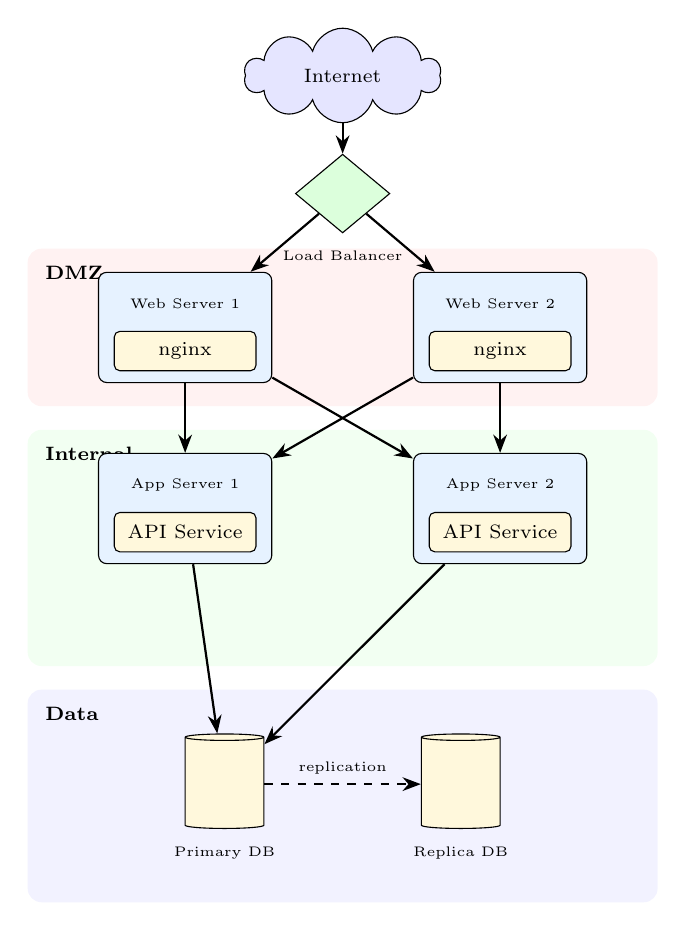
\begin{tikzpicture}[
    node distance=1.2cm and 2cm,
    server/.style={draw, fill=nodecolor, rounded corners=3pt, minimum width=2.2cm, minimum height=1.4cm},
    artifact/.style={draw, fill=componentcolor, rounded corners=2pt, minimum width=1.8cm, minimum height=0.5cm, font=\scriptsize},
    db/.style={draw, fill=componentcolor, cylinder, shape border rotate=90, aspect=0.35, minimum height=1.2cm, minimum width=1cm},
    lb/.style={draw, fill=connectorcolor, diamond, minimum width=1.2cm, minimum height=1cm},
    zone/.style={draw, dashed, rounded corners=5pt, inner sep=12pt},
    arrow/.style={-{Stealth}, thick},
    label/.style={font=\scriptsize}
]
    % Internet
    \node[draw, cloud, fill=blue!10, cloud puffs=10, minimum width=2.5cm, minimum height=1.2cm] (internet) at (0, 5) {};
    \node[font=\scriptsize] at (0, 5) {Internet};
    
    % Load Balancer
    \node[lb] (lb) at (0, 3.5) {};
    \node[font=\tiny, below=0.1cm of lb] {Load Balancer};
    
    % DMZ Zone
    \begin{scope}[on background layer]
        \fill[red!5, rounded corners=5pt] (-4, 0.8) rectangle (4, 2.8);
    \end{scope}
    \node[font=\scriptsize\bfseries, anchor=north west] at (-3.9, 2.7) {DMZ};
    
    % Web Servers
    \node[server] (web1) at (-2, 1.8) {};
    \node[font=\tiny] at (-2, 2.1) {Web Server 1};
    \node[artifact] at (-2, 1.5) {nginx};
    
    \node[server] (web2) at (2, 1.8) {};
    \node[font=\tiny] at (2, 2.1) {Web Server 2};
    \node[artifact] at (2, 1.5) {nginx};
    
    % Internal Zone
    \begin{scope}[on background layer]
        \fill[green!5, rounded corners=5pt] (-4, -2.5) rectangle (4, 0.5);
    \end{scope}
    \node[font=\scriptsize\bfseries, anchor=north west] at (-3.9, 0.4) {Internal};
    
    % App Servers
    \node[server] (app1) at (-2, -0.5) {};
    \node[font=\tiny] at (-2, -0.2) {App Server 1};
    \node[artifact] at (-2, -0.8) {API Service};
    
    \node[server] (app2) at (2, -0.5) {};
    \node[font=\tiny] at (2, -0.2) {App Server 2};
    \node[artifact] at (2, -0.8) {API Service};
    
    % Database Zone
    \begin{scope}[on background layer]
        \fill[blue!5, rounded corners=5pt] (-4, -5.5) rectangle (4, -2.8);
    \end{scope}
    \node[font=\scriptsize\bfseries, anchor=north west] at (-3.9, -2.9) {Data};
    
    % Databases
    \node[db] (db1) at (-1.5, -4) {};
    \node[font=\tiny, below=0.1cm of db1] {Primary DB};
    
    \node[db] (db2) at (1.5, -4) {};
    \node[font=\tiny, below=0.1cm of db2] {Replica DB};
    
    % Connections
    \draw[arrow] (internet) -- (lb);
    \draw[arrow] (lb) -- (web1);
    \draw[arrow] (lb) -- (web2);
    \draw[arrow] (web1) -- (app1);
    \draw[arrow] (web1) -- (app2);
    \draw[arrow] (web2) -- (app1);
    \draw[arrow] (web2) -- (app2);
    \draw[arrow] (app1) -- (db1);
    \draw[arrow] (app2) -- (db1);
    \draw[arrow, dashed] (db1) -- (db2) node[midway, above, font=\tiny] {replication};
    
\end{tikzpicture}
\caption{Three-Tier Web Application Deployment}
\end{figure}

\textbf{Description:} This example shows a classic three-tier architecture deployed across three security zones. The DMZ hosts web servers accessible from the internet through a load balancer. Application servers reside in the internal zone, and databases are isolated in a dedicated data zone with primary-replica replication.

\subsection{Example 2: Kubernetes Microservices Deployment}

\begin{figure}[H]
\centering
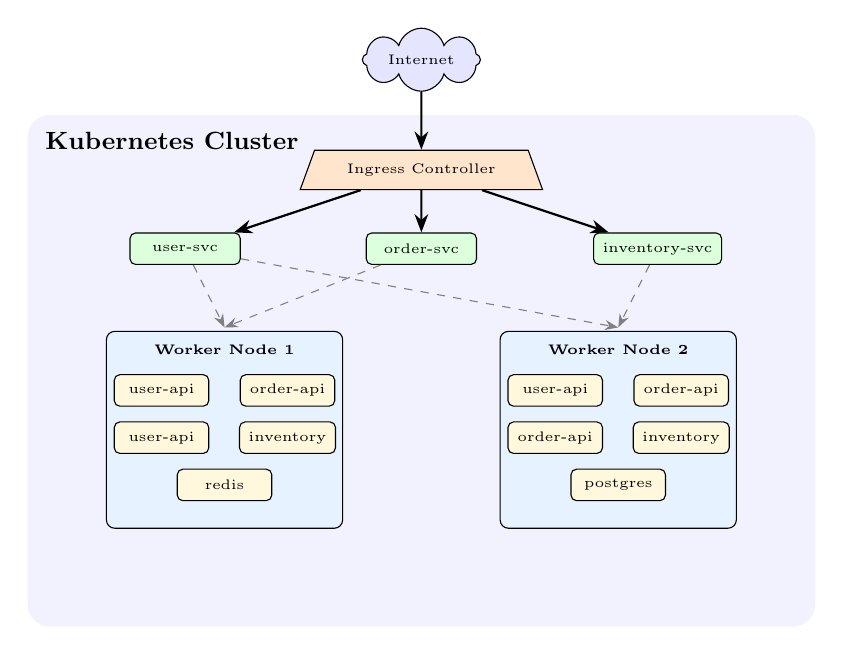
\begin{tikzpicture}[
    node distance=0.8cm and 1.5cm,
    cluster/.style={draw, thick, rounded corners=8pt, inner sep=15pt, dashed},
    node_k8s/.style={draw, fill=nodecolor, rounded corners=3pt, minimum width=3cm, minimum height=2.5cm},
    pod/.style={draw, fill=componentcolor, rounded corners=2pt, minimum width=1.2cm, minimum height=0.4cm, font=\tiny},
    service/.style={draw, fill=connectorcolor, rounded corners=2pt, minimum width=1.4cm, minimum height=0.4cm, font=\tiny},
    ingress/.style={draw, fill=orange!20, trapezium, trapezium angle=70, minimum width=1.2cm, minimum height=0.5cm, font=\tiny}
]
    % Cluster boundary
    \begin{scope}[on background layer]
        \fill[blue!5, rounded corners=8pt] (-5, -3) rectangle (5, 3.5);
    \end{scope}
    \node[font=\small\bfseries, anchor=north west] at (-4.9, 3.4) {Kubernetes Cluster};
    
    % Ingress
    \node[ingress] (ingress) at (0, 2.8) {Ingress Controller};
    
    % Services
    \node[service] (svc1) at (-3, 1.8) {user-svc};
    \node[service] (svc2) at (0, 1.8) {order-svc};
    \node[service] (svc3) at (3, 1.8) {inventory-svc};
    
    % Worker Nodes
    \node[node_k8s] (worker1) at (-2.5, -0.5) {};
    \node[font=\tiny\bfseries, anchor=north] at (-2.5, 0.7) {Worker Node 1};
    
    \node[node_k8s] (worker2) at (2.5, -0.5) {};
    \node[font=\tiny\bfseries, anchor=north] at (2.5, 0.7) {Worker Node 2};
    
    % Pods on Worker 1
    \node[pod] at (-3.3, 0) {user-api};
    \node[pod] at (-1.7, 0) {order-api};
    \node[pod] at (-3.3, -0.6) {user-api};
    \node[pod] at (-1.7, -0.6) {inventory};
    \node[pod] at (-2.5, -1.2) {redis};
    
    % Pods on Worker 2
    \node[pod] at (1.7, 0) {user-api};
    \node[pod] at (3.3, 0) {order-api};
    \node[pod] at (1.7, -0.6) {order-api};
    \node[pod] at (3.3, -0.6) {inventory};
    \node[pod] at (2.5, -1.2) {postgres};
    
    % Connections
    \draw[-{Stealth}, thick] (ingress) -- (svc1);
    \draw[-{Stealth}, thick] (ingress) -- (svc2);
    \draw[-{Stealth}, thick] (ingress) -- (svc3);
    
    \draw[-{Stealth}, dashed, gray] (svc1) -- (-2.5, 0.8);
    \draw[-{Stealth}, dashed, gray] (svc2) -- (-2.5, 0.8);
    \draw[-{Stealth}, dashed, gray] (svc3) -- (2.5, 0.8);
    \draw[-{Stealth}, dashed, gray] (svc1) -- (2.5, 0.8);
    
    % External
    \node[draw, cloud, fill=blue!10, cloud puffs=8, minimum width=1.5cm, minimum height=0.8cm] (ext) at (0, 4.2) {};
    \node[font=\tiny] at (0, 4.2) {Internet};
    \draw[-{Stealth}, thick] (ext) -- (ingress);
    
\end{tikzpicture}
\caption{Kubernetes Microservices Deployment}
\end{figure}

\textbf{Description:} This example depicts a microservices architecture deployed on Kubernetes. An ingress controller routes external traffic to internal services. Pods are distributed across worker nodes for high availability, with services providing stable network endpoints for pod groups.

\subsection{Example 3: Multi-Region Cloud Deployment}

\begin{figure}[H]
\centering
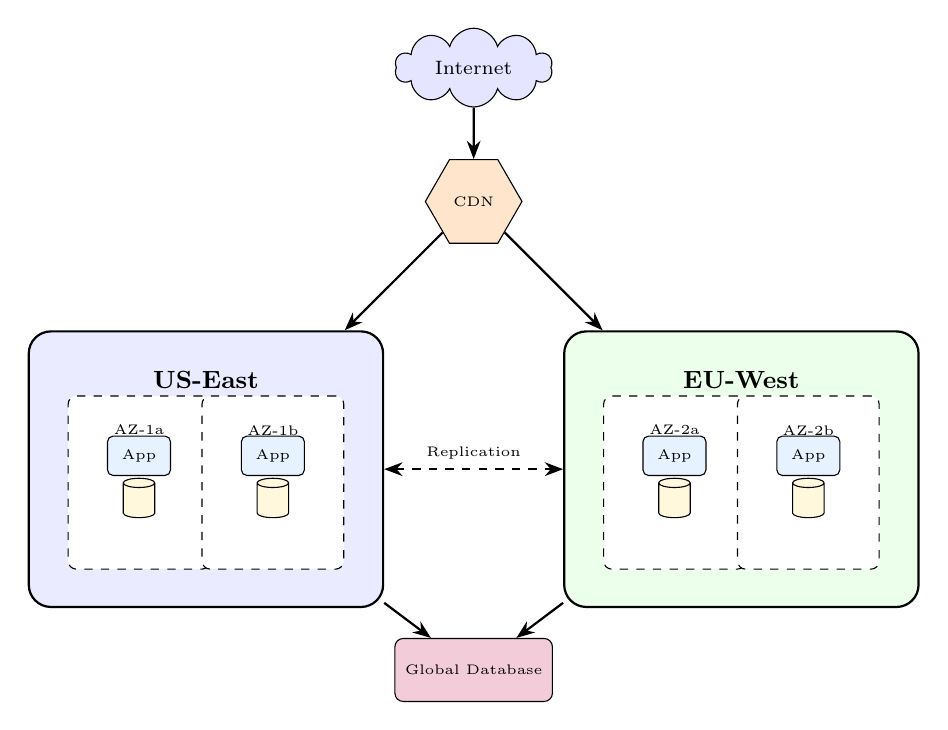
\begin{tikzpicture}[
    scale=0.85,
    region/.style={draw, thick, rounded corners=8pt, minimum width=4.5cm, minimum height=3.5cm, fill=#1},
    az/.style={draw, dashed, rounded corners=3pt, minimum width=1.8cm, minimum height=2.2cm, fill=white},
    server/.style={draw, fill=nodecolor, rounded corners=2pt, minimum width=0.8cm, minimum height=0.5cm, font=\tiny},
    db/.style={draw, fill=componentcolor, cylinder, shape border rotate=90, aspect=0.5, minimum height=0.5cm, minimum width=0.4cm},
    cdn/.style={draw, fill=orange!20, regular polygon, regular polygon sides=6, minimum size=1cm, font=\tiny}
]
    % Global CDN
    \node[cdn] (cdn) at (0, 4) {CDN};
    
    % Region US-East
    \node[region=blue!8] (useast) at (-4, 0) {};
    \node[font=\small\bfseries, anchor=north] at (-4, 1.6) {US-East};
    
    \node[az] (az1a) at (-5, -0.2) {};
    \node[font=\tiny, anchor=north] at (-5, 0.8) {AZ-1a};
    \node[server] at (-5, 0.2) {App};
    \node[db] at (-5, -0.5) {};
    
    \node[az] (az1b) at (-3, -0.2) {};
    \node[font=\tiny, anchor=north] at (-3, 0.8) {AZ-1b};
    \node[server] at (-3, 0.2) {App};
    \node[db] at (-3, -0.5) {};
    
    % Region EU-West
    \node[region=green!8] (euwest) at (4, 0) {};
    \node[font=\small\bfseries, anchor=north] at (4, 1.6) {EU-West};
    
    \node[az] (az2a) at (3, -0.2) {};
    \node[font=\tiny, anchor=north] at (3, 0.8) {AZ-2a};
    \node[server] at (3, 0.2) {App};
    \node[db] at (3, -0.5) {};
    
    \node[az] (az2b) at (5, -0.2) {};
    \node[font=\tiny, anchor=north] at (5, 0.8) {AZ-2b};
    \node[server] at (5, 0.2) {App};
    \node[db] at (5, -0.5) {};
    
    % Global Database
    \node[draw, fill=purple!20, rounded corners=3pt, minimum width=2cm, minimum height=0.8cm] (globaldb) at (0, -3) {};
    \node[font=\tiny] at (0, -3) {Global Database};
    
    % Connections
    \draw[-{Stealth}, thick] (cdn) -- (useast);
    \draw[-{Stealth}, thick] (cdn) -- (euwest);
    \draw[{Stealth}-{Stealth}, thick, dashed] (useast) -- (euwest) node[midway, above, font=\tiny] {Replication};
    \draw[-{Stealth}, thick] (useast) -- (globaldb);
    \draw[-{Stealth}, thick] (euwest) -- (globaldb);
    
    % Internet
    \node[draw, cloud, fill=blue!10, cloud puffs=10, minimum width=2cm, minimum height=1cm] (internet) at (0, 6) {};
    \node[font=\scriptsize] at (0, 6) {Internet};
    \draw[-{Stealth}, thick] (internet) -- (cdn);
    
\end{tikzpicture}
\caption{Multi-Region Cloud Deployment with Global Database}
\end{figure}

\textbf{Description:} This example shows a globally distributed deployment across two cloud regions (US-East and EU-West). Each region contains multiple availability zones for high availability. A CDN provides edge caching, and a global database service handles cross-region data consistency.

% =============================================================================
% SECTION: NOTES
% =============================================================================
\section{Notes}

\subsection{Versioning Considerations}

Deployment views should be versioned alongside the systems they document. Key versioning practices include:

\begin{itemize}
    \item Maintain separate deployment views for each environment (development, staging, production)
    \item Version deployment documentation with the software release it describes
    \item Document deltas between versions when significant changes occur
    \item Archive historical deployment configurations for audit and rollback purposes
\end{itemize}

\subsection{Tooling Recommendations}

\begin{table}[H]
\centering
\caption{Recommended Tools by Use Case}
\small
\begin{tabular}{@{}L{4cm}L{9.5cm}@{}}
\toprule
\textbf{Use Case} & \textbf{Recommended Tools} \\
\midrule
Diagram Creation & draw.io, Lucidchart, Visio, PlantUML, Structurizr \\
Infrastructure as Code & Terraform, Pulumi, AWS CDK, Azure Bicep \\
Documentation & Confluence, GitBook, Notion, Markdown/LaTeX \\
Architecture Modeling & Archi, Enterprise Architect, Structurizr \\
Cloud Visualization & Cloudcraft, Hava, Hyperglance, AWS Architecture Icons \\
Container Visualization & Lens, Octant, k9s, KubeView \\
\bottomrule
\end{tabular}
\end{table}

\subsection{Common Pitfalls}

\begin{warningbox}[Common Mistakes to Avoid]
\begin{enumerate}[nosep]
    \item \textbf{Outdated Documentation:} Deployment views that don't reflect current infrastructure lose value quickly
    \item \textbf{Excessive Detail:} Including too much low-level detail obscures important architectural decisions
    \item \textbf{Missing Security Context:} Omitting security zones and trust boundaries leaves security gaps
    \item \textbf{Single Environment Focus:} Documenting only production ignores important environment differences
    \item \textbf{No Correspondence Validation:} Failing to verify alignment with other architectural views
    \item \textbf{Static View Only:} Not documenting scaling, failover, and operational behavior
\end{enumerate}
\end{warningbox}

\subsection{Evolution and Maintenance}

Deployment documentation should be treated as a living artifact that evolves with the system:

\begin{itemize}
    \item Establish ownership and review cycles for deployment documentation
    \item Integrate deployment view updates into change management processes
    \item Automate documentation generation where possible using IaC as source of truth
    \item Conduct periodic reviews to ensure accuracy and relevance
    \item Use deployment documentation in incident post-mortems and capacity planning
\end{itemize}

% =============================================================================
% SECTION: SOURCES
% =============================================================================
\section{Sources}

\subsection{Primary References}

\begin{enumerate}
    \item Clements, P., Bachmann, F., Bass, L., Garlan, D., Ivers, J., Little, R., Merson, P., Nord, R., \& Stafford, J. (2010). \textit{Documenting Software Architectures: Views and Beyond} (2nd ed.). Addison-Wesley Professional.
    
    \item ISO/IEC/IEEE 42010:2011. \textit{Systems and software engineering --- Architecture description}. International Organization for Standardization.
    
    \item Object Management Group. (2017). \textit{Unified Modeling Language Specification Version 2.5.1}. OMG Document formal/2017-12-05.
    
    \item Brown, S. (2018). \textit{The C4 Model for Visualising Software Architecture}. Leanpub.
    
    \item The Open Group. (2022). \textit{ArchiMate 3.2 Specification}. The Open Group.
\end{enumerate}

\subsection{Supplementary References}

\begin{enumerate}[resume]
    \item Rozanski, N., \& Woods, E. (2012). \textit{Software Systems Architecture: Working with Stakeholders Using Viewpoints and Perspectives} (2nd ed.). Addison-Wesley Professional.
    
    \item Morris, K. (2020). \textit{Infrastructure as Code: Dynamic Systems for the Cloud Age} (2nd ed.). O'Reilly Media.
    
    \item Burns, B., Beda, J., \& Hightower, K. (2019). \textit{Kubernetes: Up and Running} (2nd ed.). O'Reilly Media.
    
    \item Fowler, M. (2002). \textit{Patterns of Enterprise Application Architecture}. Addison-Wesley Professional.
    
    \item Bass, L., Weber, I., \& Zhu, L. (2015). \textit{DevOps: A Software Architect's Perspective}. Addison-Wesley Professional.
\end{enumerate}

\subsection{Online Resources}

\begin{itemize}
    \item AWS Architecture Center: \url{https://aws.amazon.com/architecture/}
    \item Azure Architecture Center: \url{https://docs.microsoft.com/en-us/azure/architecture/}
    \item Google Cloud Architecture Framework: \url{https://cloud.google.com/architecture/framework}
    \item C4 Model: \url{https://c4model.com/}
    \item Kubernetes Documentation: \url{https://kubernetes.io/docs/}
\end{itemize}

% =============================================================================
% APPENDIX
% =============================================================================
\appendix

\section{Deployment View Checklist}

Use this checklist to verify completeness of deployment documentation:

\begin{table}[H]
\centering
\small
\begin{tabular}{@{}L{10cm}C{2cm}@{}}
\toprule
\textbf{Item} & \textbf{Complete?} \\
\midrule
\multicolumn{2}{l}{\textbf{Scope and Context}} \\
\quad System/subsystem clearly identified & $\square$ \\
\quad Target environments documented & $\square$ \\
\quad Stakeholders identified & $\square$ \\
\midrule
\multicolumn{2}{l}{\textbf{Infrastructure Elements}} \\
\quad All nodes documented with specifications & $\square$ \\
\quad Network topology defined & $\square$ \\
\quad Security zones established & $\square$ \\
\quad Storage infrastructure specified & $\square$ \\
\midrule
\multicolumn{2}{l}{\textbf{Software Allocation}} \\
\quad All artifacts mapped to nodes & $\square$ \\
\quad Runtime environments specified & $\square$ \\
\quad Dependencies documented & $\square$ \\
\quad Configurations defined per environment & $\square$ \\
\midrule
\multicolumn{2}{l}{\textbf{Quality Attributes}} \\
\quad High availability mechanisms documented & $\square$ \\
\quad Scaling approach defined & $\square$ \\
\quad Security controls specified & $\square$ \\
\quad Performance considerations addressed & $\square$ \\
\midrule
\multicolumn{2}{l}{\textbf{Operations}} \\
\quad Deployment procedures documented & $\square$ \\
\quad Monitoring integration specified & $\square$ \\
\quad Backup and recovery defined & $\square$ \\
\quad Operational runbooks available & $\square$ \\
\midrule
\multicolumn{2}{l}{\textbf{Validation}} \\
\quad Correspondence with C\&C view verified & $\square$ \\
\quad Stakeholder review completed & $\square$ \\
\quad Implementation matches documentation & $\square$ \\
\bottomrule
\end{tabular}
\end{table}

\section{Glossary}

\begin{description}[style=nextline, leftmargin=3cm, labelwidth=2.8cm]
    \item[Artifact] A deployable unit of software such as an executable, library, container image, or configuration file.
    
    \item[Availability Zone] A physically separate location within a cloud region, providing isolation from failures in other zones.
    
    \item[Container] A lightweight, standalone executable package that includes everything needed to run software.
    
    \item[Deployment] The process of making software available for use on target infrastructure.
    
    \item[Environment] A complete set of infrastructure and configuration for running software (e.g., development, staging, production).
    
    \item[Failover] The automatic switching to a redundant system upon failure of the primary system.
    
    \item[High Availability] A characteristic of systems designed to be operational for a high percentage of time.
    
    \item[Infrastructure as Code] The practice of managing infrastructure through machine-readable definition files.
    
    \item[Load Balancer] A device or service that distributes network traffic across multiple servers.
    
    \item[Node] A computational resource capable of hosting and executing software.
    
    \item[Pod] The smallest deployable unit in Kubernetes, consisting of one or more containers.
    
    \item[Region] A geographic area containing one or more data centers operated by a cloud provider.
    
    \item[Replication] The process of copying data between nodes to ensure consistency and availability.
    
    \item[Security Zone] A network segment with defined security policies and trust levels.
    
    \item[Scaling] The ability to increase or decrease resources to handle varying workloads.
    
    \item[Virtual Machine] A software emulation of a physical computer that runs an operating system.
\end{description}

% =============================================================================
% END DOCUMENT
% =============================================================================

\end{document}s